%%%%%%%%%%%%%%%%%%%%%%%%%%%%%%%%%%%%%%%%%%%%%%%%%%%%%%%%%%%%%%
%%%%		PLANTILLA LATEX PARA INFORMES
%%%%			LATEX REPORT TEMPLATE
%%%%
%%%%	Autor	: Carlos Gonzalez Cortes
%%%%	Correo	: carlgonz@ug.uchile.cl
%%%%	Version	: 1.0
%%%%
%%%%	Notas	: Este codigo se entrega tal cual es y sin
%%%%			  ningun tipo de garantia. Sientase libre de
%%%%			  modificar y compartir.(acentos omitidos en
%%%%			  los comentarios por compatibilidad)
%%%%
%%%%%%%%%%%%%%%%%%%%%%%%%%%%%%%%%%%%%%%%%%%%%%%%%%%%%%%%%%%%%%




\documentclass[11pt,letterpaper]{article}
\usepackage[spanish]{babel}
%\usepackage[ansinew]{inputenc}
\usepackage[utf8]{inputenc}
% \usepackage[latin1]{inputenc}
\usepackage[letterpaper,includeheadfoot, top=0cm, bottom=1.5cm, right=2.0cm, left=2.0cm, headheight=77pt]{geometry}
\renewcommand{\familydefault}{\sfdefault}

\usepackage{graphicx}
\usepackage{color}
\usepackage{hyperref}
\usepackage{amssymb}
\usepackage{url}
%\usepackage{pdfpages}
\usepackage{fancyhdr}
\usepackage{hyperref}
\usepackage{subfig}
\usepackage{lmodern}
\edef\restoreparindent{\parindent=\the\parindent\relax}
\usepackage{parskip}
\restoreparindent

\usepackage{listings} %Codigo
\lstset{language=Python, tabsize=4,breaklines=true}

\definecolor{codegreen}{rgb}{0,0.6,0}
\definecolor{codegray}{rgb}{0.5,0.5,0.5}
\definecolor{codepurple}{rgb}{0.58,0,0.82}
\definecolor{backcolour}{rgb}{0.8, 0.8, 0.8}

\lstdefinestyle{mystyle}{
    %backgroundcolor=\color{backcolour},
    commentstyle=\color{codegreen},
    keywordstyle=\color{magenta},
    numberstyle=\tiny\color{codegray},
    stringstyle=\color{codepurple},
    basicstyle=\footnotesize,
    breakatwhitespace=false,
    breaklines=true,
    captionpos=t,
    keepspaces=true,
    numbers=left,
    numbersep=8pt,
    showspaces=false,
    showstringspaces=false,
    showtabs=false,
    tabsize=4
}

\usepackage{xcolor}

\colorlet{punct}{red!60!black}
\definecolor{background}{HTML}{EEEEEE}
\definecolor{delim}{RGB}{20,105,176}
\colorlet{numb}{magenta!60!black}

\lstdefinelanguage{json}{
    literate=
     *{0}{{{\color{numb}0}}}{1}
      {1}{{{\color{numb}1}}}{1}
      {2}{{{\color{numb}2}}}{1}
      {3}{{{\color{numb}3}}}{1}
      {4}{{{\color{numb}4}}}{1}
      {5}{{{\color{numb}5}}}{1}
      {6}{{{\color{numb}6}}}{1}
      {7}{{{\color{numb}7}}}{1}
      {8}{{{\color{numb}8}}}{1}
      {9}{{{\color{numb}9}}}{1}
      {:}{{{\color{punct}{:}}}}{1}
      {,}{{{\color{punct}{,}}}}{1}
      {\{}{{{\color{delim}{\{}}}}{1}
      {\}}{{{\color{delim}{\}}}}}{1}
      {[}{{{\color{delim}{[}}}}{1}
      {]}{{{\color{delim}{]}}}}{1},
}

\lstset{style=mystyle}


% footnote in footer
\newcommand{\fancyfootnotetext}[2]{%
  \fancypagestyle{dingens}{%
    \fancyfoot[LO,RE]{\parbox{12cm}{\footnotemark[#1]\footnotesize #2}}%
  }%
  \thispagestyle{dingens}%
}

%images
\graphicspath{{img/}}

\begin{document}
%\begin{sf}
% --------------- ---------PORTADA --------------------------------------------
\newpage
\pagestyle{fancy}
\fancyhf{}
%-------------------- CABECERA ---------------------
\fancyhead[L]{ 
\includegraphics[scale=0.3]{img/fcfm_dcc.pdf} }
%\fancyhead[R]{ 
\includegraphics[scale=0.4]{img/fcfm.png} }
%------------------ TÍTULO -----------------------
\vspace*{6cm}
\begin{center}
\Huge  {Informe de Práctica}\\
\vspace{1cm}
\small {CC5901 -- Práctica Profesional II}\\
\end{center}
%----------------- NOMBRES ------------------------
\vfill
\begin{flushright}
\begin{tabular}{ll}
Empresa: & Departamento de Ingeniería Eléctrica\\
        & Universidad de Chile \\
Supervisor: & Sandra Céspedes, Ph.D.\\
Alumno: & Manuel Olguín\\
Carrera: & Ingeniería Civil en Computación\\
RUT:& 18.274.982 -- 6\\
E-Mail: & molguin@dcc.uchile.cl\\
Tel: & +56 9 7463 6997\\
& \today\\
& Santiago, Chile.
\end{tabular}
\end{flushright}

% ·············· ENCABEZADO - PIE DE PAGINA ············
\newpage
\pagestyle{fancy}
\fancyhf{}

%Encabezado
%\fancyhead[L]{\rightmark}
%\fancyhead[L]{\small \rm \textit{Sección \rightmark}} %Izquierda
%\fancyhead[R]{\small \rm \textbf{\thepage}} %Derecha

\fancyfoot[L]{\small \rm \textit{Sección \rightmark}} %Izquierda
\fancyfoot[R]{\small \rm \textbf{\thepage}} %Derecha

%\fancyfoot[L]{\small \rm \textit{Pie de página - Izquierda}} %Izquierda
%\fancyfoot[R]{\small \rm \textit{Pie de página - Derecha}} %Derecha
%\fancyfoot[C]{\thepage} %Centro

\renewcommand{\sectionmark}[1]{\markright{\thesection.\ #1}}
\renewcommand{\headrulewidth}{0.5pt}
\renewcommand{\footrulewidth}{0.5pt}

\newpage
\section{Certificado de la Empresa}
\newpage
\section{Observaciones}
\newpage
% =============== INDICE ===============

\tableofcontents
\listoffigures

% =============== SECCION ===============
\newpage
\section{Resumen}

El presente documento detalla el trabajo realizado entre Agosto y Octubre del 2016 por el alumno Manuel Olguín en el Grupo de Investigación en Wireless Networking del Departamento de Ingeniería Eléctrica de la Universidad de Chile. Dicho trabajo se realizó bajo la supervisión de la profesora Sandra Céspedes, y consistió en la modelación de un sistema de alarma temprana para ciclistas en el contexto de un Sistema de Transporte Inteligente.

\newpage
\section{Introducción}
\subsection{Lugar de Trabajo}

El Grupo de Investigación en Wireless Networking (en adelante, \emph{el Grupo}) es un conjunto de estudiantes y profesionales del área de Tecnologías de la Información y Comunicaciones (en adelante, \emph{TICs} \cite{TICS}) liderado por la profesora Sandra Céspedes \cite{scespedes}, docente del Departamento de Ingeniería Eléctrica de la Universidad de Chile (en adelante, \emph{DIE} \cite{DIE}). El Grupo desarrolla sus labores de investigación y desarrollo en el Laboratorio de Comunicaciones Avanzadas, ubicado en el 5\textsuperscript{o} piso del departamento del DIE ubicado en Av. Tupper 2007, Santiago.

\subsection{Equipo de Trabajo}

Los miembros del grupo son estudiantes de pre- y posgrado, además de profesionales ligados a las TICs, de diversos orígenes, especialidades e incluso nacionalidades. En específico, el trabajo realizado por el practicante fue desarrollado bajo la supervisión de la doctora Sandra Céspedes y en colaboración con un estudiante de pregrado del DIE.

\newpage
\subsection{Software y Conceptos Importantes}

El trabajo se realizó principalmente en C++ y Python, utilizando software especializado para la modelación y estudio de redes inalámbricas, redes de transporte y la integración de ambas en Sistemas de Transporte Inteligente.

\subsubsection{Sistemas de Transporte Inteligente}

Los sistemas de transporte conforman la columna vertebral de nuestras ciudades, contribuyendo directamente al desarrollo de la sociedad urbana. Un sistema de transporte bien diseñado y eficiente permite el desplazamiento rápido y cómodo de personas y bienes; en cambio, uno ineficiente genera grandes problemas, alargando los tiempos de viaje y aumentando la contaminación atmosférica.

Los Sistemas de Transporte Inteligente (en adelante \emph{ITS}, por sus siglas en inglés -- \textit{Intelligent Transportation Systems}) surgen como una respuesta a la necesidad de optimización y modernización de los sistemas de transporte existentes. La Unión Europea define a los ITS como aplicaciones avanzadas que, sin incorporar inteligencia como tal, pretenden proveer servicios innovadores relacionados con distintos modos de transporte y de administración de tráfico, que además otorgan información a los usuarios, permitiéndoles utilizar el sistema de transporte de manera más segura, coordinada e inteligente \cite{eudirective}. De acuerdo al Departamento de Transportes de los EEUU, estos sistemas se pueden dividir en dos grandes categorías \cite{usdot}:
\begin{description}
  \item [Sistemas de Infraestructura Inteligente] Tienen como enfoque el manejo de los sistemas de transporte a niveles macro, y la transmisión de información oportuna a los usuarios. Esta categoría incluye, entre otros, sistemas de advertencia y señalización dinámica en ruta (ya sea a través de pantallas o sistemas de comunicación inalámbrica), sistemas de pago electrónico y de coordinación del flujo de tráfico.

  \item [Sistemas de Vehículos Inteligentes] Engloba todo aquello relacionado con la automatización y optimización de la operación de un vehículo. Dentro de esta categoría se incluyen sistemas de advertencia y prevención de colisiones, de asistencia al conductor --- por ejemplo, sistemas de navegación --- y control autónomo de vehículos.

\end{description}

El factor común entre ambas categorías es la necesidad de extraer información en tiempo real desde el entorno, la cual debe procesarse y en muchos casos generar una respuesta a transmitir al usuario. Para este fin, actualmente se utilizan tecnologías de comunicación inalámbricas, tanto de área local (los estándares incluídos en la familia WLAN, IEEE 802.11), como de área personal (WPAN, IEEE 802.15) \cite{80211dailey,80215vanet,80211wave}.

\subsubsection{OMNeT++}

\emph{Objective Modular Network Testbed in C++}, mejor conocido como OMNeT++ \cite{omnet}, es un \emph{framework} y librería para la simulación de sistemas de eventos discretos, principalmente utilizado para la simulación y análisis de redes de comunicaciones. Consiste en un conjunto de módulos y librerías en C++, además de un entorno de desarrollo integrado (en adelante, \emph{IDE} por sus siglas en inglés -- \emph{Integrated Development Environment}) y una interfaz gráfica, los cuales posibilitan la construcción de simulaciones dinámicas y extensibles tanto de sistemas cableados como inalámbricos.

OMNeT++ es software libre, de fuente abierta, y altamente popular en la comunidad académica.


\begin{figure}[ht]
  \centering
  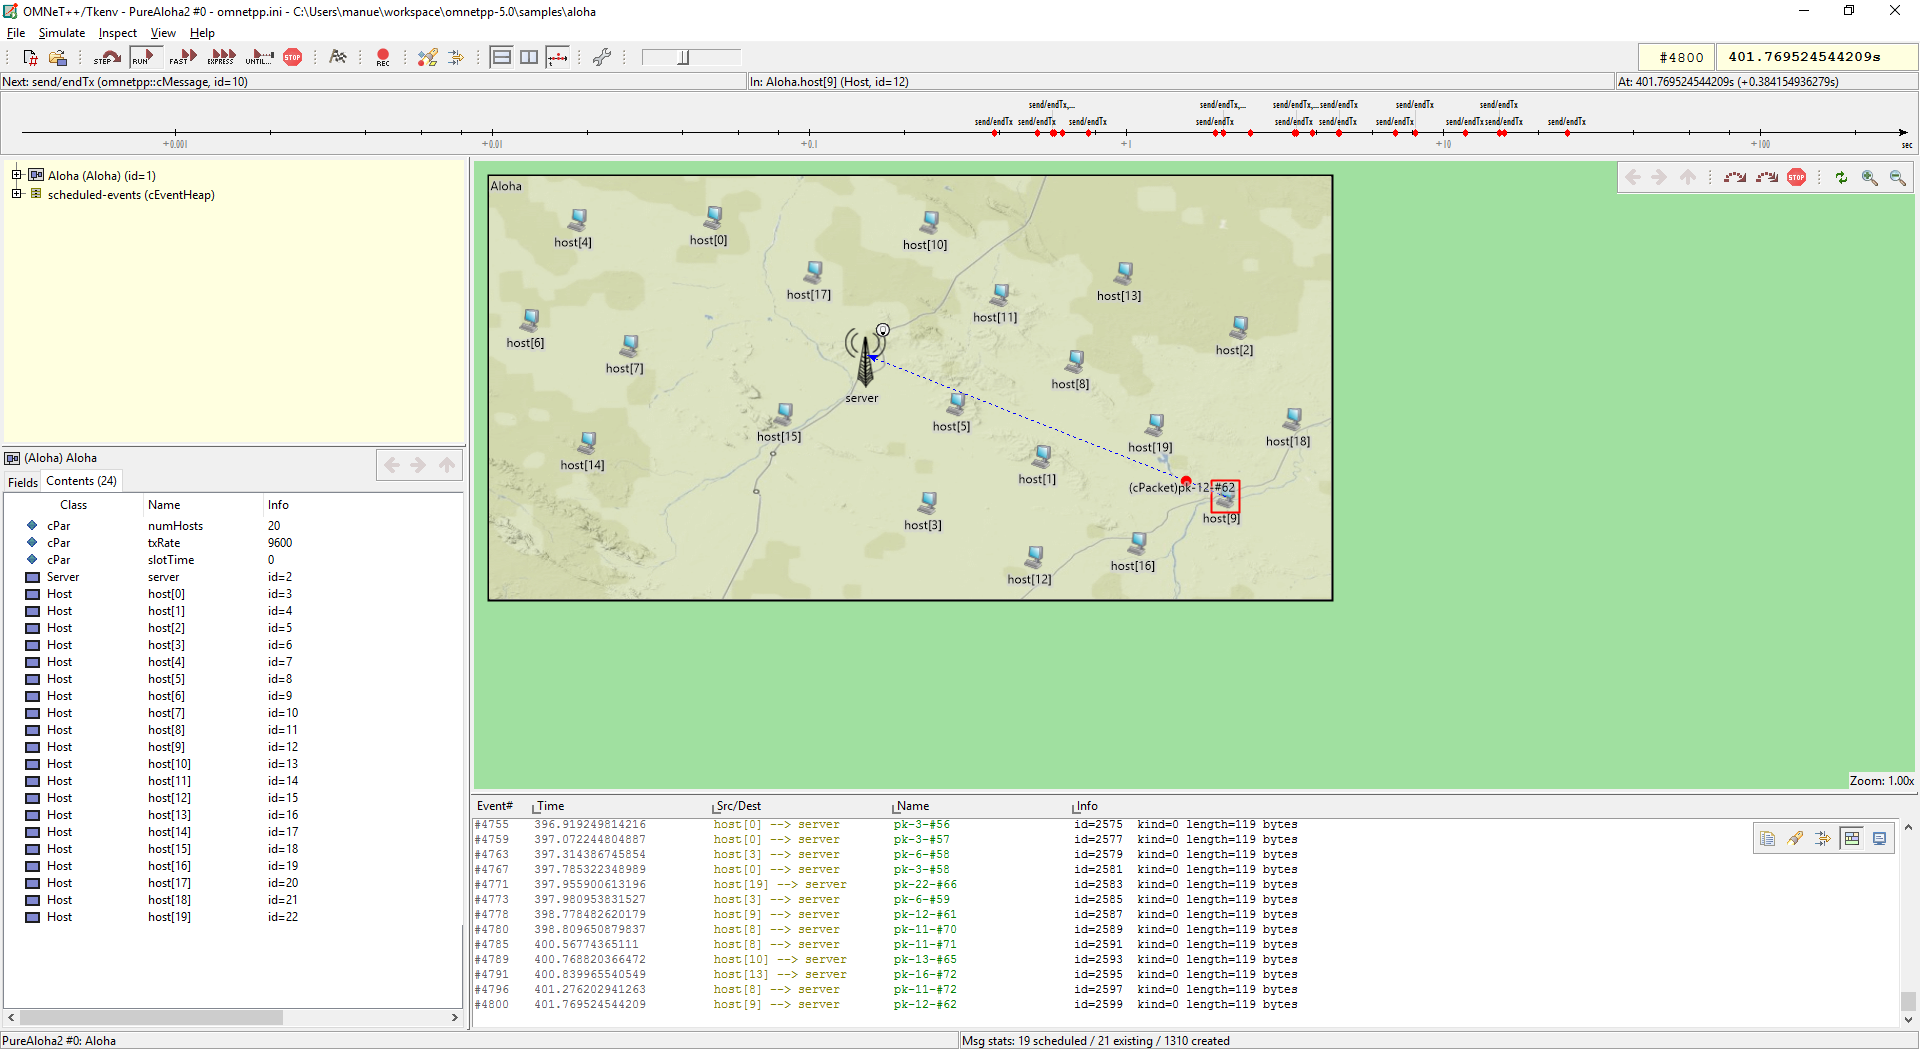
\includegraphics[width=\linewidth]{aloha.png}
  \caption{Entorno gráfico de simulación de OMNeT++}
  \label{fig:omnetgui}
\end{figure}

\subsubsection{SUMO}

SUMO (\emph{Simulation of Urban MObility}) es un simulador de tráfico vehicular de fuente abierta desarrollado originalmente por el Instituto de Sistemas de Transporte del Centro Aeroespacial Alemán (DLR, por sus siglas en alemán -- \emph{Deutsches Zentrum für Luft- und Raumfahrt e.V.}) \cite{sumo}. Es un simulador microscópico, en el cual cada vehículo es simulado de manera particular, moviéndose individualmente por la red.

\begin{figure}[ht]
  \centering
  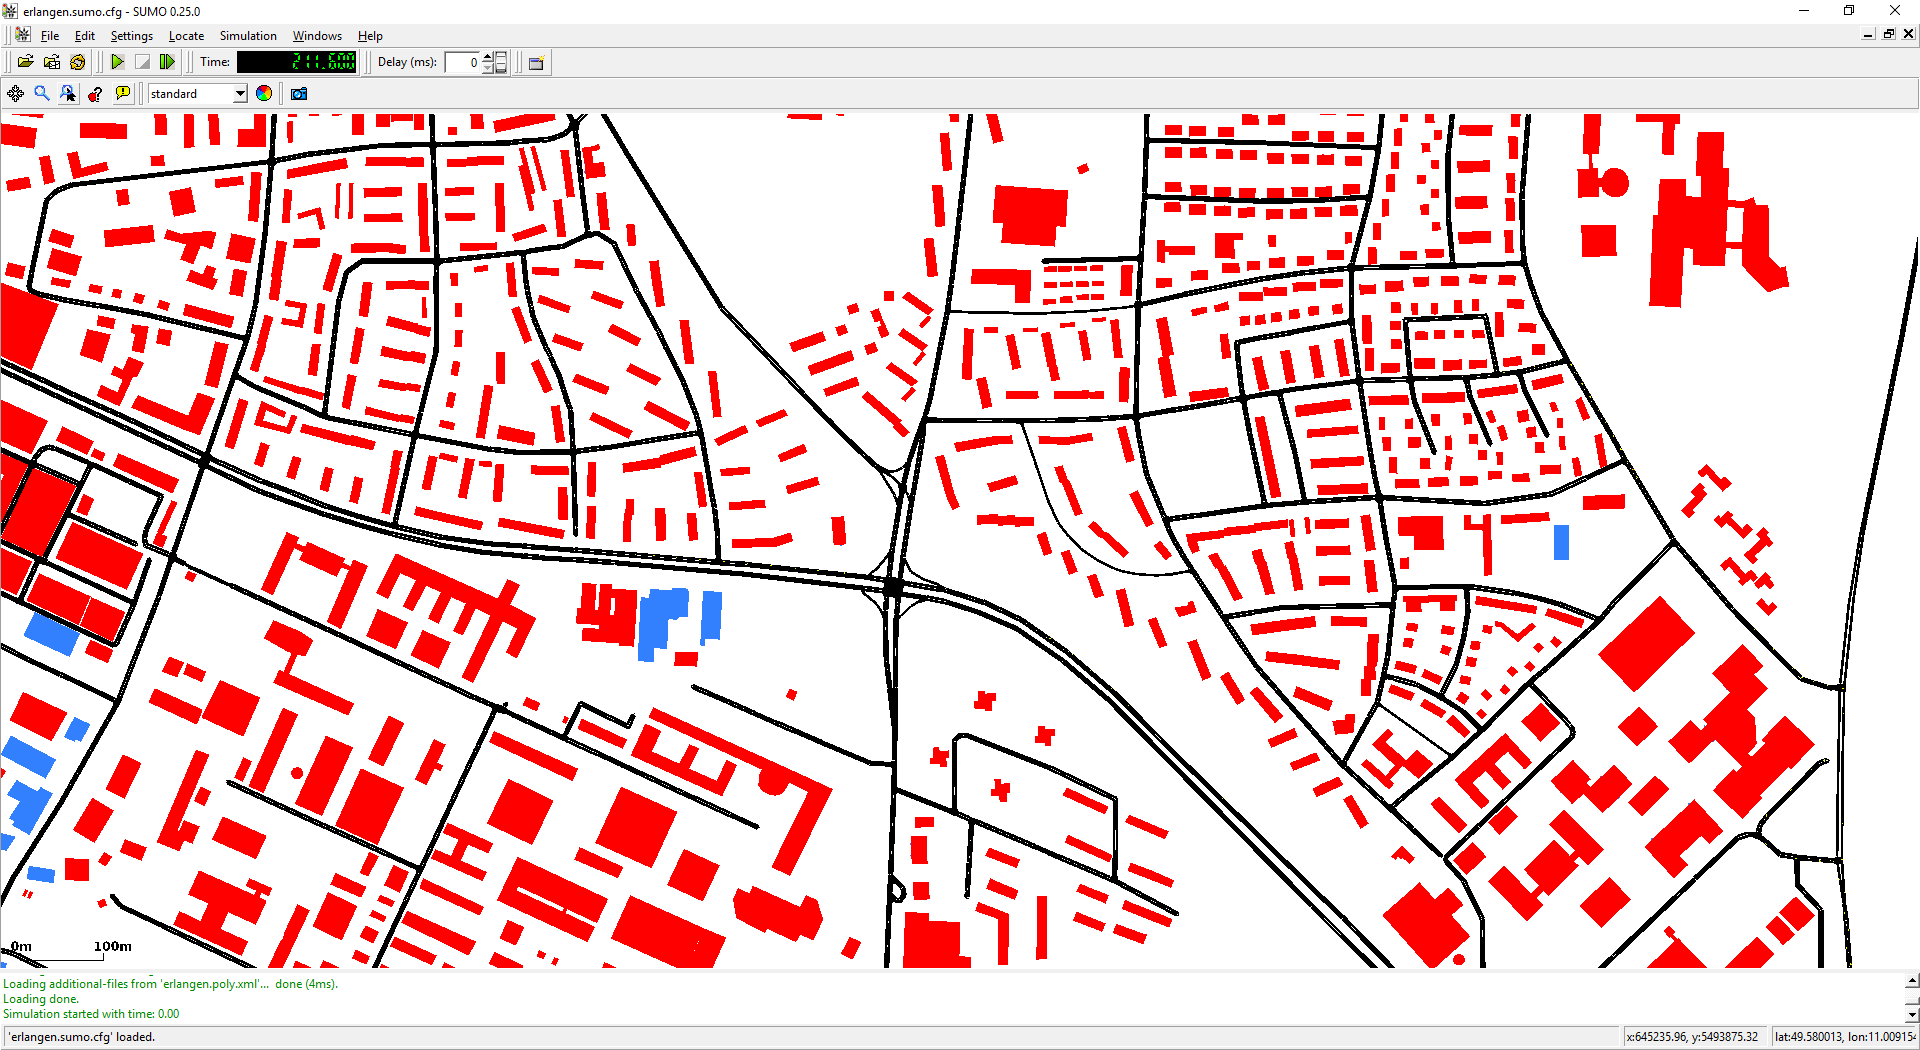
\includegraphics[width=\linewidth]{sumo_demo.png}
  \caption{Simulación de una red en SUMO}
  \label{fig:sumo_demo}
\end{figure}

\subsubsection{VEINS}

\emph{VEhicles In Network Simulation}, \emph{VEINS}, es un framework de fuente abierta para la simulación, tanto en su aspecto de comunicaciones como de transporte, de Sistemas de Transporte Inteligente.


\subsection{Situación Previa}\label{section:situacion_previa}

\newpage
\section{Trabajo Realizado}

El trabajo realizado tenía como fin último la elaboración de un prototipo de un sistema de alerta temprana para ciclistas en un ITS. El fin de este sistema era el de predecir, mediante un modelo de probabilidades bayesianas descrito por Liebner \textit{et al.} en \cite{prediction-paper}, la probabilidad de un giro sorpresivo de un vehículo en un cruce, y notificar esto a ciclistas cercanos a dicho cruce (se asumieron ciclistas y vehículos en el contexto de un ITS, dotados de capacidades de comunicación inalámbrica).

Este trabajo se dividió entonces en dos partes:

\begin{enumerate}
  \item Estudio y comprensión del software especializado OMNeT++, SUMO y VEINS, y la posterior elaboración de un prototipo simple para ilustrar la factibilidad del proyecto.
  \item Implementación del sistema, utilizando como base el prototipo anterior y utilizando registros de tráfico real.
\end{enumerate}

Cabe destacar que las labores del practicante abarcaron la implementación del modelo vehicular y la integración del modelo predictivo a este. El estudio y la implementación del modelo descrito en \cite{prediction-paper} quedó a cargo de Sebastián Piña M., alumno del DIE y compañero de equipo del practicante.

\subsection{Estudio del software y elaboración de un prototipo inicial simple}

El primer mes de la práctica se enfocó totalmente en el estudio del software especializado, enfocado principalmente en VEINS y la elaboración de modelos de sistemas de transporte inteligentes utilizando el framework. Esto además significó el aprendizaje de C++ por parte del practicante. Con el fin de realizar un aprendizaje didáctico y aplicado, se implementó además un prototipo simple de un cruce vehicular con carriles para ciclistas.

\subsubsection{Prototipo inicial}

El prototipo inicial se construyó en base al trabajo previamente realizado por Javiera Born (descrito en la sección \ref{section:situacion_previa}). Este consistió en una simulación muy simple, compuesta por un vehículo motorizado y una bicicleta, los cuales interactúan en un cruce. A continuación se detalla la elaboración de este prototipo, y los resultados obtenidos para la siguiente etapa del trabajo de práctica.

\begin{figure}[ht]
  \centering
  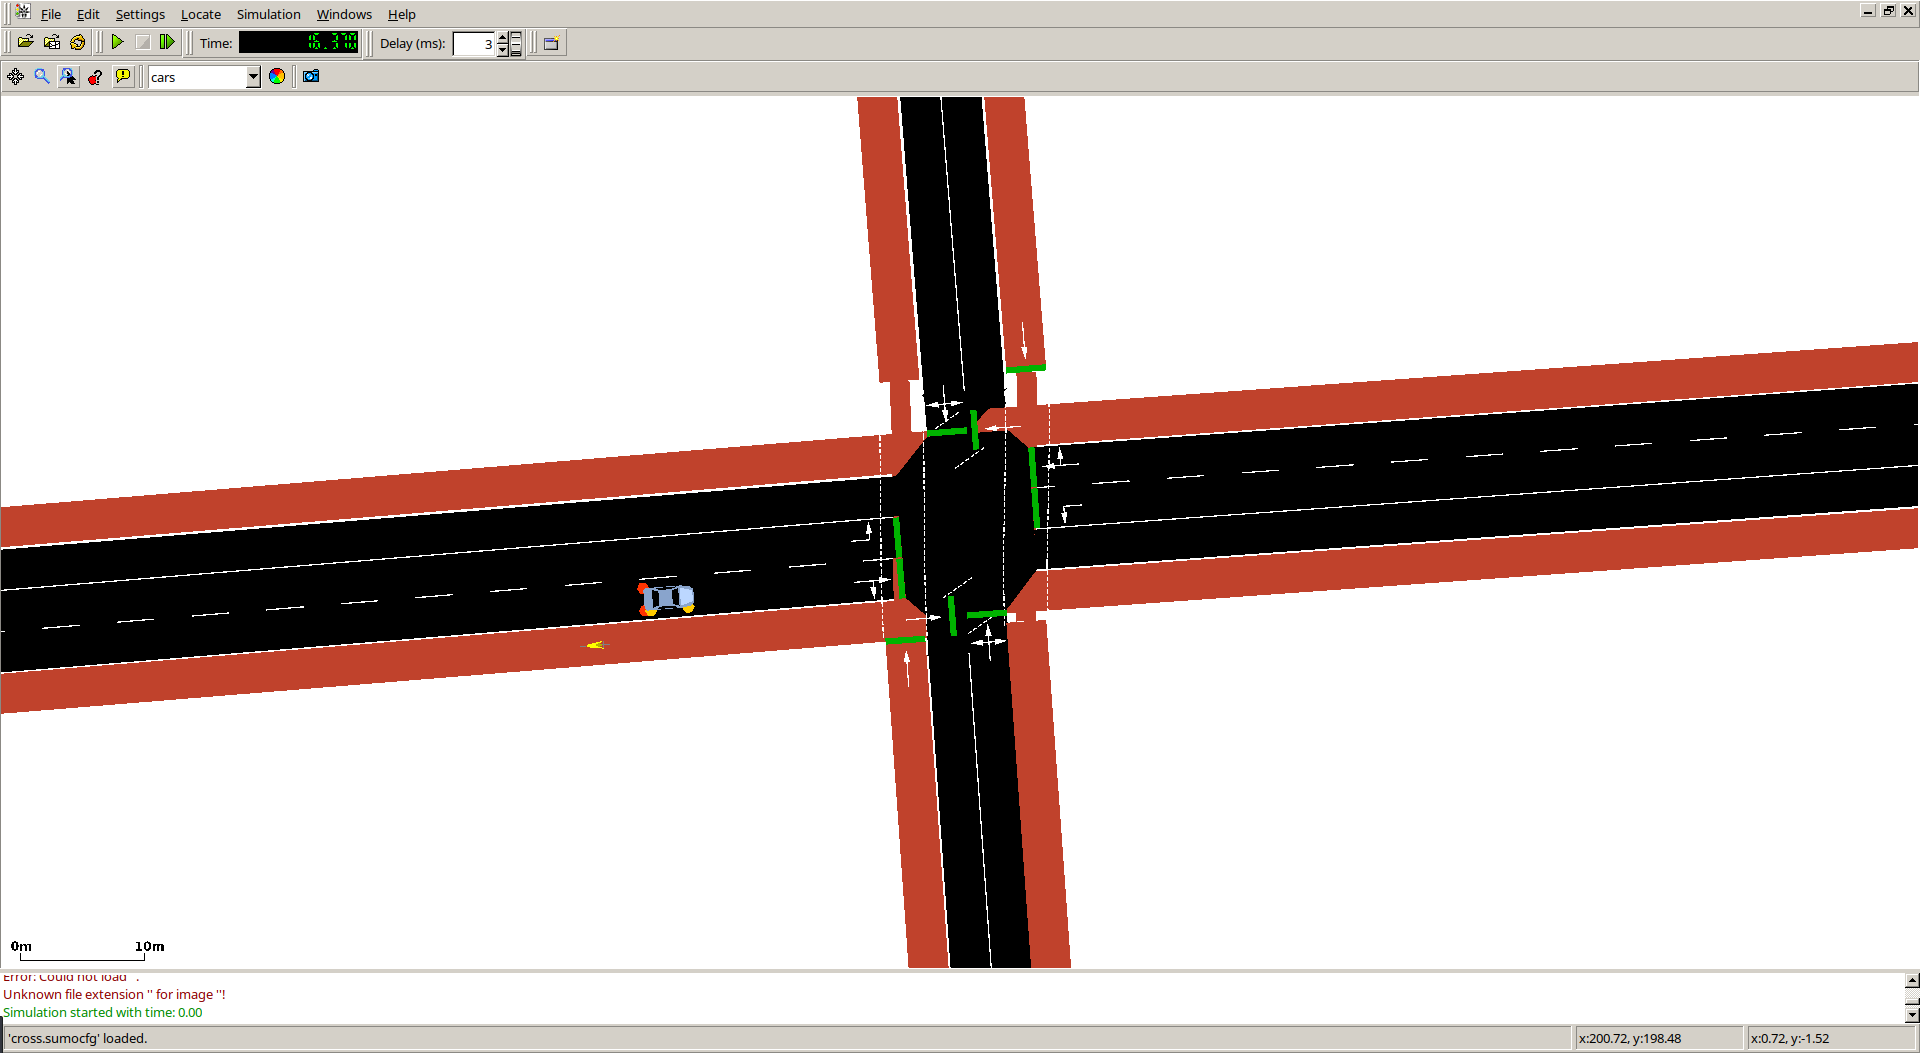
\includegraphics[width=\linewidth]{prototipo_inicial.png}
  \caption{Prototipo inicial en ejecución}
  \label{fig:sumo_prototype}
\end{figure}

\subsubsection{Parámetros físicos de la simulación}

El aspecto de transporte de la simulación no presenta grandes cambios respecto a lo desarrollado anteriormente por J. Born -- se reutilzó el cruce vehicular simple compuesto por una vía de tres pistas y otra de dos, ambas con ciclovías a los costados. Se modificaron los flujos vehiculares para que consistieran únicamente en un automóvil y una bicicleta, y para sincronizar su llegada al cruce y poder simular la detención de la bici en reacción a un mensaje de viraje emitido por el automóvil (detalles de la implementación de esto en la sección \ref{section:prot_communication}).

\subsubsection{Simulación de comunicación inalámbrica y lógica?}\label{section:prot_communication}

La lógica de la simulación se implementó en un módulo de OMNeT++ llamado \emph{BikeManeuver}. En este módulo se implementó el comportamiento de ambos vehículos (automóvil y bicicleta), diferenciando su comportamiento durante la ejecución mediante un \emph{flag} seteado al inicio de la simulación.

El comportamiento de ambos es muy simple, pero sirve para ilustrar y entender el comportamiento de VEINS.



\newpage
\section{Conclusiones}
\newpage
\begin{thebibliography}{5}
    \bibitem{TICS} \emph{Tecnologías de la Información y Comunicaciones} - \url{https://es.wikipedia.org/wiki/Tecnolog%C3%ADas_de_la_informaci%C3%B3n_y_la_comunicaci%C3%B3n}

    \bibitem{scespedes} \emph{Sandra Céspedes U.} - \url{http://www.cec.uchile.cl/~scespedes/}

    \bibitem{DIE} \emph{Departamento de Ingeniería Eléctrica} - \url{http://die.cl/}

    \bibitem{eudirective}
  		\hbadness=1000 Directive 2010/40/EU of the European Parliament and of the Council
  		\textit{on the framework for the deployment of Intelligent Transport Systems in the field of road transport and for interfaces with other modes of transport},
  		2010 O.J. L 207/1

    \bibitem{usdot}
  		\hbadness=1000 U.S. Department of Transportation
  		\textit{Office of the Assistant Secretary for Research and Technology (OST-R)}
  		\\\url{http://www.itsoverview.its.dot.gov/} (\textit{04/2017})

    \bibitem{80211dailey}
  		\hbadness=1000 D. J. Dailey, K. McFarland and J. L. Garrison
  		\textit{Experimental study of 802.11 based networking for vehicular management and safety},
  		Intelligent Vehicles Symposium (IV), 2010 IEEE, San Diego, CA, 2010, pp. 1209-1213.
  		\\doi: 10.1109/IVS.2010.5547955


  	\bibitem{80215vanet}
  		\hbadness=1000 W. Xiong; X. Hu; T. Jiang.
  		\textit{Measurement and Characterization of Link Quality for IEEE 802.15.4-compliant Wireless Sensor Networks in Vehicular Communications},
  		IEEE Transactions on Industrial Informatics , vol.PP, no.99, pp.1-1
  		\\doi: 10.1109/TII.2015.2499121

  	\bibitem{80211wave}
  		\hbadness=1000 D. Jiang and L. Delgrossi.
  		\textit{IEEE 802.11p: Towards an International Standard for Wireless Access in Vehicular Environments}, Vehicular Technology Conference, 2008. VTC Spring 2008. IEEE, Singapore, 2008, pp. 2036-2040.
  		\\doi: 10.1109/VETECS.2008.458

    \bibitem{omnet}
  		\hbadness=1000 OMNeT++ Discrete Event Simulator.
  		\textit{An extensible, modular, component-based C++ simulation library and framework, primarily for building network simulators}.
  		\\\url{https://OMNeTpp.org/} (\textit{04/2017})

    \bibitem{sumo}
  		\hbadness=1000 SUMO – Simulation of Urban MObility.
  		\textit{A free and open traffic simulation suite which is available since 2001.}
  		\\\url{http://sumo.dlr.de} (\textit{4/2017})

    \bibitem{prediction-paper}
      \hbadness=1000 M. Liebner, F. Klanner, M. Baumann, C. Ruhhammer and C. Stiller.
      \textit{Velocity-Based Driver Intent Inference at Urban Intersections in the Presence of Preceding Vehicles},
      IEEE Intelligent Transportation Systems Magazine, vol. 5, no. 2, pp. 10-21, Summer 2013.
      \\doi: 10.1109/MITS.2013.2246291

\end{thebibliography}


% ============= FIN DE DOCUMENTO ==============
\end{document}
